\documentclass[a4paper,10pt]{scrartcl}
\usepackage[utf8]{inputenc}
\usepackage{enumerate,graphicx}
\usepackage[ngerman]{babel}

\begin{document}

\begin{center}
  \Huge Hardwarepraktikum \\
  \large Andre Löffler, Fabian Helmschrott, Nils Wisiol \\
  \today
\end{center}


\section*{Aufgabe A}

\subsection*{Aufgabe 1}
\begin{enumerate}
 \item Um die Aufgabe zu lösen, haben wir die Unterdiagramme mit Hifle \texttt{subplot} und entsprechenden Parametern geplottet. 

Die wesentliche Information der Signale befindet sich im Frequenzbereich der menschlichen Sprache, also ca. 100 bis 5000 Hz. Die Unterschiede zwischen den Aufnahmen sind, dass die Kinderstimme besonders hohe Frequenzen erzeugt, nämlich bis zu 7kHz, während Gandalf besonders niedrige Frequenz verwendet, nämlich um 100Hz.
\begin{figure}[h]
 \centering
 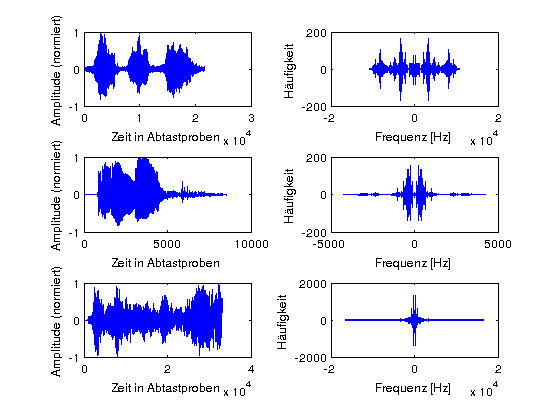
\includegraphics[width=.8\textwidth]{./Bilder/A/1_1.png}
 % 1_1.png: 560x420 pixel, 90dpi, 15.81x11.85 cm, bb=0 0 448 336
\end{figure}

Beispielaufruf: \texttt{aufgabeA1} gibt das in der Abbildung gezeigte Bild aus.
 \item Um hohe Frequenzen zu löschen, haben wir eine Fouriertransformation durchgeführt, die hohen Bereiche mit 0 überschrieben und anschließend eine Rücktransformation vorgenommen. Dabei wurden komplexe Werte durch ihren reellen Betrag ersetzt. 

Die Qualität sinkt im allgemeinen, da Informationen verloren gehen. \texttt{run.wav} ist mit 3,5kHz noch verständlich. \texttt{ring.wav} ist mit 1,5kHz noch verständlich. \texttt{aloha.wav} ist mit 1kHz noch verständlich. Ausblenden geht bei \texttt{run.wav} einfach, da die Hintergrundgeräusche hochfrequent sind.

Beispielaufruf: \texttt{aufgabeA2(3000)} gibt \texttt{aloha.wav} zuerst ungefiltert, danach nur mit Frequenzen kleiner 3000 Hz aus.
 \item Zum Resampling liegt der Algorithmus das alte und das neue Abtastgitter übereinander. Direkt passende Werte werden übernommen, Werte an neuen Abtastpunkten, die zwischen zwei alten Abtastpunkten liegen, werden mit Hilfe von \texttt{interp1} interpoliert. 

Erhöhung in ein Vielfaches: keine Änderung. Sonstige Erhöhung: geringfügige Verschlechterung durch Interpolation. Verringerung: Verschlechterung durch Verlust von Information. Eine Überabtastung liegt bei Erhöhung der Abtastrate vor, denn dann können Frequenzen erfasst werden, die vorher nicht erfasst werden konnten. Eine Unterabtastung liegt bei Verringerung der Abtastrate vor, wenn zuvor hochfrequente Signale gespeichert wurden. Die Dateigröße ist proportional zur Abtastrate.

Beispielaufruf: \texttt{aufgabeA3(.5,3500)} spielt \texttt{run.wav} zuerst ungefiltert, dann mit Frequenzen kleiner 3500 Hz, dann zusätzlich mit halber Samplingrate ab. 
 \item Das Signal wird mit Hilfe der Treppenfunktion \(\lfloor x \cdot n \rfloor / n \) quantisiert.

Man benötigt 2 bit bei \texttt{run.wav}, 3 bit bei \texttt{ring.wav}, 3 bit bei \texttt{aloha.wav}. Eine Beurteilung gestaltet sich schwierig, da die Samples bereits aus den vorherigen Aufgaben bekannt sind und so sehr leicht wiedererkannt werden können.
\begin{figure}[h]
 \centering
 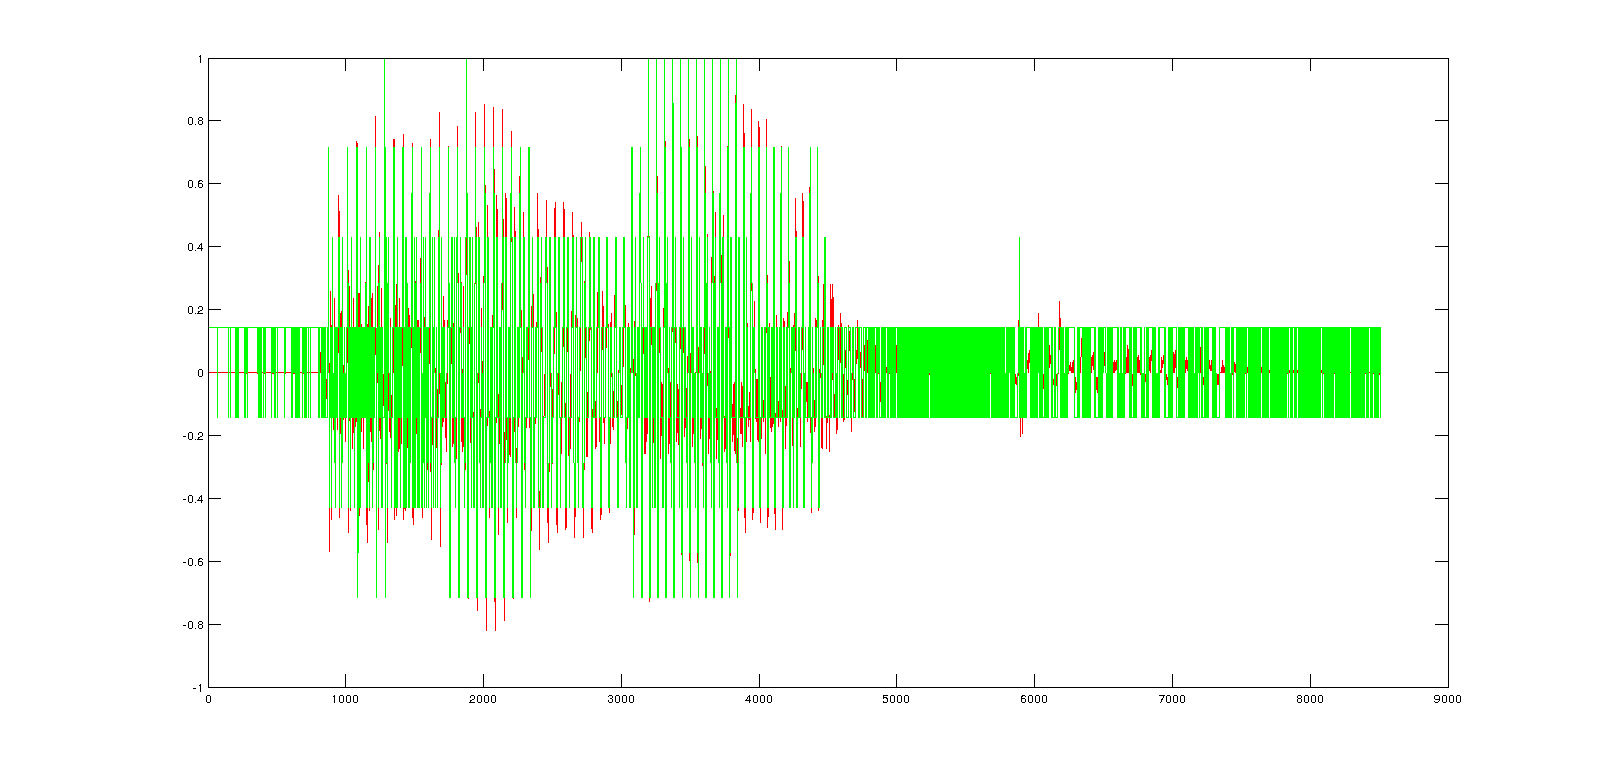
\includegraphics[width=0.8\textwidth]{./Bilder/A/1_4.png}
 % 1_4.png: 1600x772 pixel, 90dpi, 45.16x21.79 cm, bb=0 0 1280 618
\end{figure}

Beispielaufruf: \texttt{aufgabeA4(3)} spielt \texttt{aloha.wav} auf \(2^3 = 8\) Quantisierungsstufen ab.
  \item Die SQNR verbessert sich im Allgemeinen um 6 dB pro zusätzliches bit und variiert leicht bei unterschiedlichen Sprechern. 
\begin{figure}[h]
 \centering
 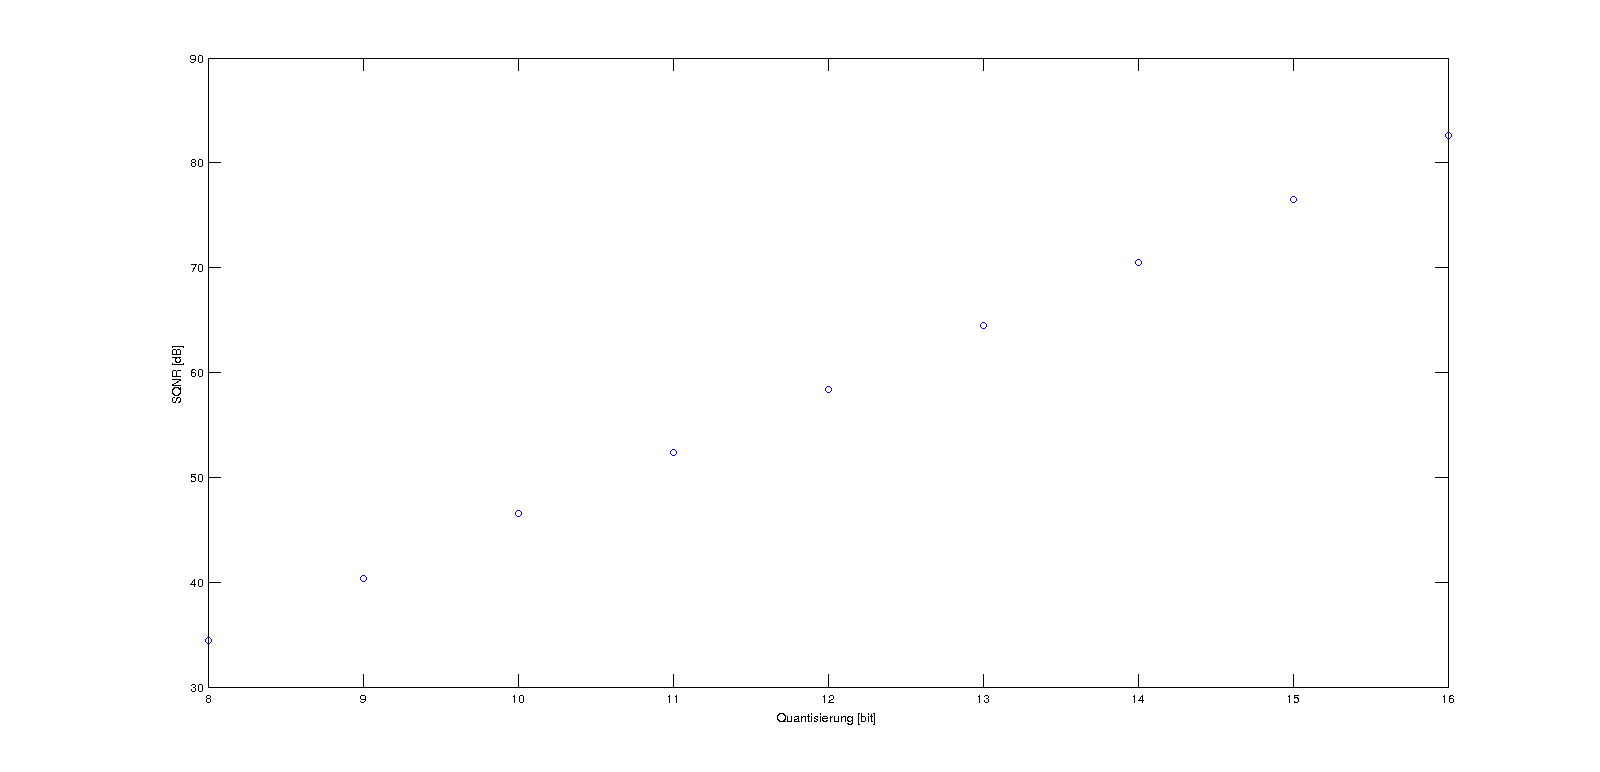
\includegraphics[width=0.8\textwidth]{./Bilder/A/1_5.png}
 % 1_5.png: 1600x772 pixel, 90dpi, 45.16x21.79 cm, bb=0 0 1280 618
\end{figure}

Beispielaufruf: \texttt{aufgabeA5} spielt \texttt{ring.wav} mit 8 kHz Abtastrate und plottet das entsprechende Quantisierungs-SQNR-Diagramm.
  \item Die modifizierte \texttt{linquant()}-Funktion wurde als \texttt{linquantmod} gespeichert.  
\end{enumerate}

\subsection*{Aufgabe 2}
\begin{enumerate}
  \item Die Funktion implementiert die rekursive Definition.

Beispielaufruf: \texttt{walsh(16)} 
  \item Spreizung: Erzeugung von \(n\) bits aus einem bit des Klartextes mittels Multiplakation mit dem Spreading-Vektor. De-Spreizung: Erzeugung von einem Bit aus \(n\) bits des Codeworts mittels Skalarmultiplikation und Division durch die Anzahl an 1-bits im Spreadingcode.

Beispielaufruf: \texttt{despread(spread([-1 -1 1], [1 1 -1]),[1 1 -1])'} entspreizt das Gespreizte und liefert am Ende wieder die Eingabe.

  \item Beispielaufruf: \texttt{aufgabeA23(0)} spielt zuerst das vorbereitete Signal ab, danach das übertragene Signal.
  \item 

Ja, der Fehler macht sich bemerkbar. Hörbare Verschlechterung bereits bei 1\% Fehlerwahrscheinlichkeit, völlig unverständlich bei 10\% (Codelänge: 4). Bei einer Codelänge von 64 bit tritt keine oder kaum eine Verschlechterung des Signals ein, da diese Codes eine höhere Redundanz (größere Hamming-Distanz) haben.

Beispielaufruf: \texttt{aufgabeA23(0.01)} spielt zunächst das vorbereitete Signal ab, danach das mit 1\% Fehlerwahrscheinlichkeit und Codelänge 4 bit Übertragene. 
 \item Signale der anderen sind vom starken Signal überlagert. Dies kann prinzipiell auch in der Realität auftreten, daher sollte man die Signale nochmals für jeden Teilnehmer verschlüsseln. Bei UMTS teilt die Zelle dem Empfänger mit, wie laut er senden soll.

Beispielaufruf: \texttt{aufgabeA25} überträgt \texttt{run.wav} mit Sendegewinn 7 und spielt dann die empfangenen Signale nacheinander ab.
\end{enumerate}

\subsection*{Aufgabe 3}
\begin{enumerate}
 \item Das Codewort für \texttt{1010} lautet \texttt{1010110}.

Beispielaufruf: \texttt{schieberegisterHamming([1 0 1 0])}
 \item Die allgemeine Implementierung ist in allen Fällen schneller. Die erzeugten Codeworte waren immer gleich.

Beispielaufruf: \texttt{aufgabeA32} vergleicht die Zeiten und gibt die Differenz aus.
 \item Solange die höchste Potenz des Dividenten größer ist als die des Divisors, wird deren Differenz mutlipliziert mit dem Divisor vom Dividenten abgezogen. Dies entspricht genau der Polynomdivision, am Ende ist der Divident gerade der Rest. Dabei ist zur Vereinfachung der Implementierung das höchstwertige Bit im Vektor ganz rechts notiert.

Man erhält \texttt{1010011}

Beispielaufruf: \texttt{polydiv([0 1 0 1],[1 1 0 1],7)} berechnet das gesuchte Codewort.
 \item Bei der ersten Folge wurde kein Bit verfälscht, bei der zweiten Folge wurde das letzte Bit verfälscht. Die Restfehlerwahrscheinlichkeit beträgt laut Informationsübertragung-Skript
	\[ p_{RK} = 1 - \sum_{i=0}^\eta { n \choose i } p_b^i(1-p_b)^{n-i} = 1 - { n \choose 0 } p_b^0(1-p_b)^n - { n \choose 1 } p_b (1-p_b)^{n-1} = \]
	\[ = 1 - (1 - p_b)^n - n p_b (1-p_b)^{n-1} \]
	Für \(p_b = 0,01\) ergibt sich also eine Restfehlerwahrscheinlichkeit von \(0,002\) und für \(p_b = 0,001\) eine von \(2 \cdot 10^{-5}\). Das erste Wort wird als fehlerfrei erkannt, beim zweiten Wort wird ein Fehler an der fünften Stelle erkannt.

Beispielaufruf: \texttt{meggitDecodierer([1 0 1 0 1 1 0], [1 1 0 1])}
 \item Fehlertyp 2 verursacht weniger Störungen, geringere Bitfehlerwahrscheinlichkeit sorgt für bessere Übertragung. In unserer Implementierung mussten wir \texttt{wavplay} durch \texttt{sound} ersetzen, da \texttt{wavplay} nicht Linux-kompartibel ist.

Beispielaufruf: \texttt{aufgabeA35}
\end{enumerate}

\end{document}
